%!TEX root = ../dissertation.tex
\begin{savequote}[75mm]
``In the end, you're measured not by how much you undertake but by what you
finally accomplish"
\qauthor{Donald Trump - POTUS}
\end{savequote}

\chapter{Evaluation}
This chapter will provide a critical evaluation of the projects journey and
the deliverables that were produced. In terms of following a method each
deliverable will be evaluated using my manifesto (Section
\ref{sec:manifesto}) and the following questions:
\begin{enumerate}
\item Did it meet the requirements? How?
\item How could it be improved? Why?
\item What impact did it make?
\item What the future holds
\end{enumerate}

\section{A11Y Guide}
\subsection{Meeting requirements}
This section will evaluate against the requirements set out in section
\ref{sec:requirements} and will describe success and/or shortcomings.

\begin{center}
\textit{``I want to have a section highlighting the most important aspects I
need to take on board"}
\end{center}
I am satisfied that this requirement has been fulfilled. After an
introductory paragraph each piece of guidance has an 'Essentials' section
which documents the most important things developers should do. This is then followed
by a collection of resources to allow users to gain a deeper understanding.
\begin{figure}[H]
\centering
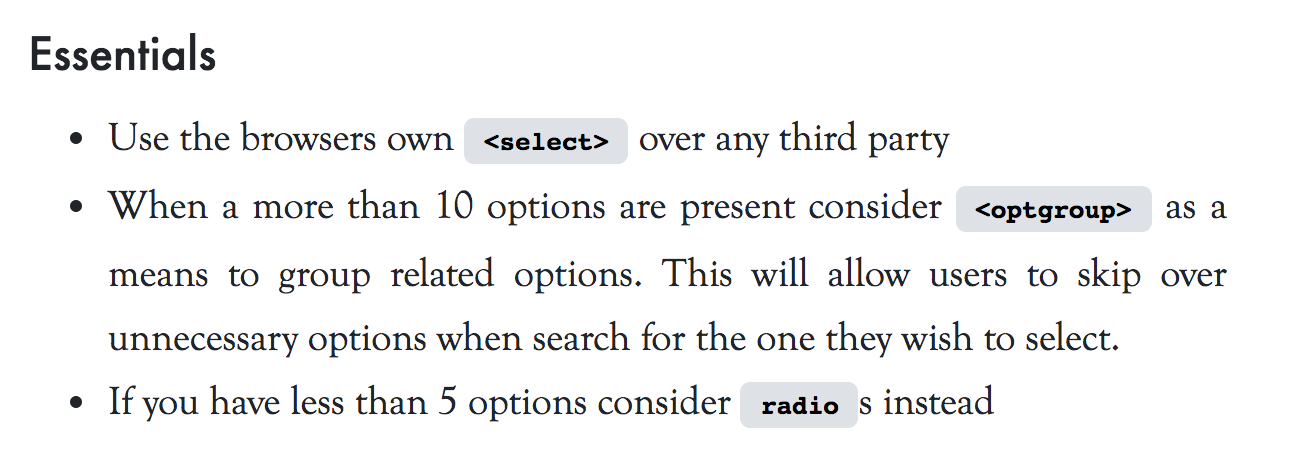
\includegraphics[width=0.6\textwidth]{figures/guide_essentials}
\captionsetup{justification=centering}
\caption{`Essentials' section for select menus
\label{fig:guide_essentials}}
\end{figure}

\begin{center}
\textit{``I want to have coded examples written in React"}
\end{center}
Due to the nature of the topic this requirement is difficult to
measure. Most of the examples written used react as a means to demonstrate
good and bad practice. An improvement that I worked in during Iteration 4 was
to enable the documentation framework to embed examples. This was really
impactful as it enables developers to see the code, the result, and the
snippet of the tool.
A problem I had was it was difficult to pitch a `component' at the write
level for users as I was
unsure what they would do with it. Would they use it as is? Would they just
take the HTML? Would they just read and understand it? Perhaps some additional
research into how users would use the coded examples would have allowed for
more meaningful examples.

\begin{center}
\textit{``I want to have assistive tool examples of different markups"}
\end{center}
This was implemented mainly through subtitles in the side bar as shown in Fig
.~\ref{fig:a11y_guide_assistive_tool_snippet}. I felt it demonstrated really well the difference
in what applying good semantics can make to the experience of assistive
tools. The deliverable faultered in demonstrating tools other than those for
the visually/motor impaired. By including examples from other tools a richer
understanding could have been given.

\begin{figure}[H]
\centering
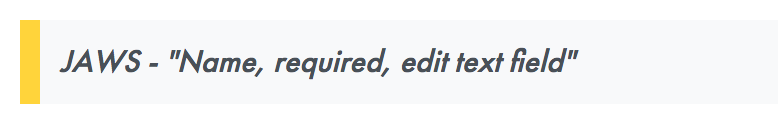
\includegraphics[width=0.6\textwidth]{figures/a11y_guide_assistive_tool_snippet}
\captionsetup{justification=centering}
\caption{Example of JAWS snippet for input's
\label{fig:a11y_guide_assistive_tool_snippet}}
\end{figure}


\begin{center}
\textit{``I want relevant links available"}
\end{center}
I feel this requirement was fully satisfied. For every part of the guide a
collection of at least three useful links was included. Because I followed a
method for collecting the resources (Section \ref{sec:GatheringKnowledge}) and
in many cases used them myself to understand various topics I am confident
that thier content is of high quality.

In hindsight assessing each link in this way was extremely time consuming and
resulted in only slightly better content. But it means the guide makes a good
reference document for each topic.

\subsection{Impact}
\subsubsection{Personal \& Business}
From a personal level I have found this deliverable extremely useful! I
actively use the content and best practices it documents in most of my day to
day work. When discussing with colleagues accessibility and my expertise on
accessibility I have been able to refer to this to backup claims and
suggestions I make.

From a business perspective the guide targets the frameworks and components
which are used across current Capgemini projects. The real impact will
only be seen as a greater period of time goes by. Tom Brown a 'Test lead` said
the following about the guide and its contents.

\begin{center}
\textit{``The guide gives a great overview of how to fix the common issues we
often identify during assistive tool testing. Typically when we show developers
how the tools behave they are keen to fix the problems they have made. It is
good to see the demosntrations of how the tools behave."}
\end{center}

Being an employee of Capgemini and this work been available in the public
domain it is possible that this work will result in a reputation gain as
Capgemeni being a 'leader' in accessible research and writing inclusive
software.

\subsection{Future}
The conclusion of this project will not be the end of the guide. I plan on
adding more content and using it as a means of demonstrating my skills to the
wider development community and potential employers.

\section{A11Y Tool}
Similar to the A11Y Guide this section will evaluate against the requirements
defined in section \ref{ref:requirements}

\subsection{Meeting requirements}
\begin{center}
\textit{I want to be able to customise the ruleset}
\end{center}
Through the introduction of `checker packs' this requirement has been
achieved. A checker pack is defined through a single Javascript which uses
ES6 import statements although realtively clean an alternate 'nicer' way in
which these could have been achieved was through a json file

\begin{center}
\textit{I want to be able to run the tool through multiple methods}
\end{center}
Evidence of this being possible is relatively limited but the high level
design of the tool demonstrates how it could be done. With A11Y Core being
seperate to A11Y Browser wrapping the core module in a CLI runner for tools
like jenkins should relatively easy.

\begin{center}
\textit{I want to be able to have errors categorised}
\end{center}
The A11Y core module returns all results from every checker. Error, Warning,
Info and Success. It is then up to the consuming module to handle these. The
A11Y Browser module filters this list to only contain Errors and Warnings and
then displays them in a `report' to the user as demonstrated in
Fig.~\ref{fig:a11y_tool_report}. Inline with many other applications Yellow
means warning and Red means error.

\begin{figure}[H]
\centering
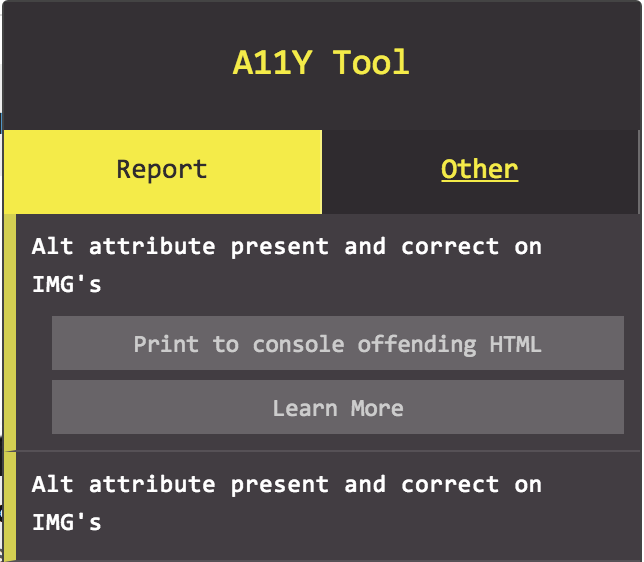
\includegraphics[width=0.6\textwidth]{figures/a11y_tool_report}
\captionsetup{justification=centering}
\caption{Report generated by the A11Y Browser module
\label{fig:a11y_tool_report}}
\end{figure}

\begin{center}
\textit{I want remediation advice to have more information}
\end{center}
The important aspect to evaluate here is that A11Y Core enables a means and
recommends a way of setting remediation advice for issues found. This
requirement has been satisfied by extending the Result object and adding
remediation to it. `Checker's written by users are expected to add the remedy
to the problem they have identified.

\subsection{Next time}
Due to the lost time I was only able to complete two iterations on the A11Y
Tool in comparison to the six on the A11Y Guide. I feel this reflects in both
the report and product produced. The design feels sound, but the product
relatively immature.

If I were to deliver this project again with the same incidents and time
constraints I would probably have changed direction and aimed for only a
single deliverable the `A11Y guide'.

\subsection{Impact}
As mentioned above time was relatively tight towards the end of the project
and thus it has had little time to make an impact across Capgemini and the
wider development community.

\subsection{Future}
With the work that has gone into designing/developing the tool thus far I
believe the ideas and implementation are extensible and could sit as an
alternative to some of the more well known tools. Following this project I am
hoping to continue its development into a more solid product.


\section{Extending the impact}
With one of my manifest items being ``Make an impact over getting a good
grade" I was looking for opportunities throughout the project to extend this.
Below I have documented some additional deliverables which came out of the
project as direct side effects of the work done.

\subsection{Colour Contrast Tool}
\label{sec:colour_contrast}
Whilst I was creating the A11Y Guide I was asked to experiment with an
upcoming piece of technology. ``CSS in JS" \citep{CSSInJS}. The industry has been moving
towards `component driven' development \citep{CDD} through the entrance of
Angular
and ReactJS; CSS in JS is the last step in all code relating to a
component being co-located in a single file. Myself like others had had
significant reservations \citep{AgainstCssInJs} about the performance and portability of
such an idea. However, working for a technology consultancy firm we are
advised to form an opinion on any impacting changes within our retrospective
spaces.

Having done research into colour contrast tools as part of the A11Y Guide I
identified a gap for a ``modern", user focussed tool. Most current tools
require submission to a server and lack demonstrations
of what the two colours look like when used together \cite*{JuicyStudio}. All
of them satisfied a relatievly simple set of requirements:
\begin{itemize}
\item Report the colour contrast level between two distinct colours
\item Report whether the colours contrast level of such colours satisfies the
 WCAG guidelines for the ``wanted" text size.
\end{itemize}

Using Moqups \citep{Moqups} I quickly put together a quick design using
their colour schemes and fonts See \ref{fig:colour_contrast_1}. To test out
``CSS in JS" I wanted to use `Styled Components' a ReactJS implementation
written by \cite*{StyledComponents} which has gained real traction. ``Create
React App" was again used to speed up the development process. This was
only an `experiment' and thus to be completed quickly, testing was reduced to
cover only the core logic for calculating colour contrast.

\begin{figure}[H]
\centering
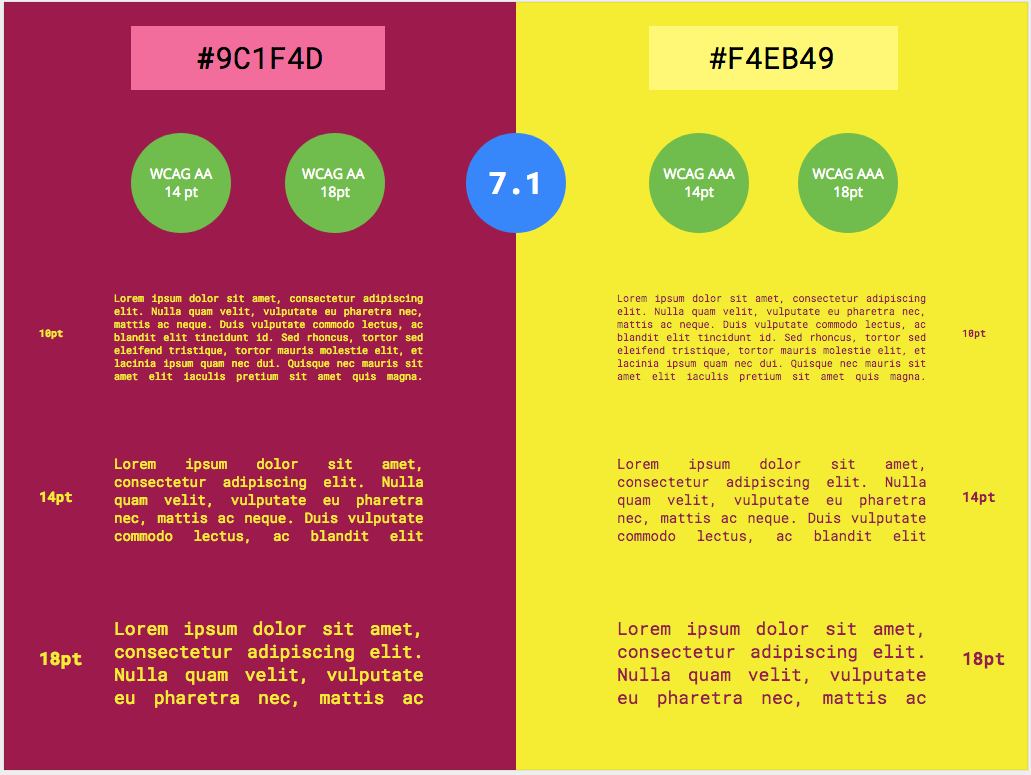
\includegraphics[width=0.65\textwidth]{figures/colour_contrast_1}
\captionsetup{justification=centering}
\caption{Design for Colour Contrast tool
\label{fig:colour_contrast_1}}
\end{figure}

The `Happy Day' user journey would be:
\begin{itemize}
\item User enters first colour in input field (Can paste)
\item User enters second colour in input field
\item On a valid colour entered. Both are displayed as background and
foreground; the value of colour contrast is displayed; and the contrast
levels WCAG appropriateness is displayed in the circles. Green for success, Red
for failure.
\end{itemize}

In the error scenario of a user entering an invalid colour, the background
colours would remain the same and the input field would have a `red'
background and border to signify an error.

This was deployed through github pages to \url{https://colour-contrast.github.io/}
and was tweeted about by myself and
subsequently the creator of 'styled-components'. In the month
the tool has been live it has gained \textasciitilde450 views across most
countries. It receives \textasciitilde3-4 views a day now.

\begin{figure}[H]
\centering
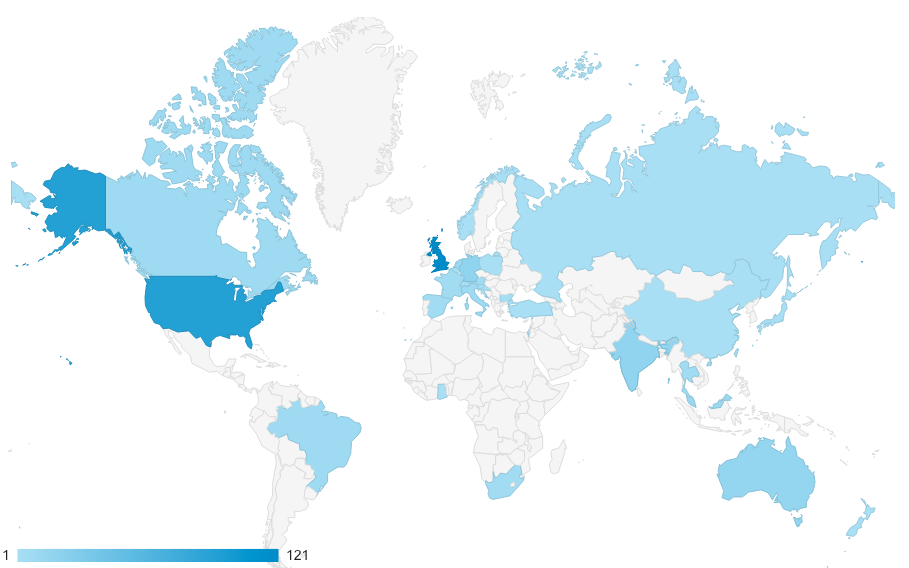
\includegraphics[width=0.65\textwidth]{figures/colour_contrast_analytics}
\captionsetup{justification=centering}
\caption{Google Analytics location based viewing statistics
\label{fig:colour_contrast_analytics}}
\end{figure}


\section{Ways of working}
This is an area of the project which probably experienced the most
experimentation, problems and successes.

\subsection{Project Diary}
`Medium' was used to blog the journey and significant events that
occured throughout the project. I did this to produce a level of transparency
between myself, my supervisors and the wider Capgemini community. In
acheiving that goal I think it did a great job. To start with each post was
targetted towards individual items of `progress' with titles such as 'The
Manfesto' and `Snapshot of web frameworks'. However, I realised that this
wasn't really a `diary' of events that happened and would not be sufficient
to fulfil the role of the project diary.

I decided to change the format into a weekly update
detailing a summary of what happened followed by in depth notes about
anything that had been delivered that week. It was great to be able to send
these to my supervisors and helped to keep the project on track. I
think this was because commitments
made in were publically available and thus to me became higher priorty.

All blog posts are available at \url{https://medium.com/@Geeman201/}. Below
is an example of the most popular post `March 2017 - Web Framework Snapshots'
which received 42 reads alone.

\begin{figure}[H]
\centering
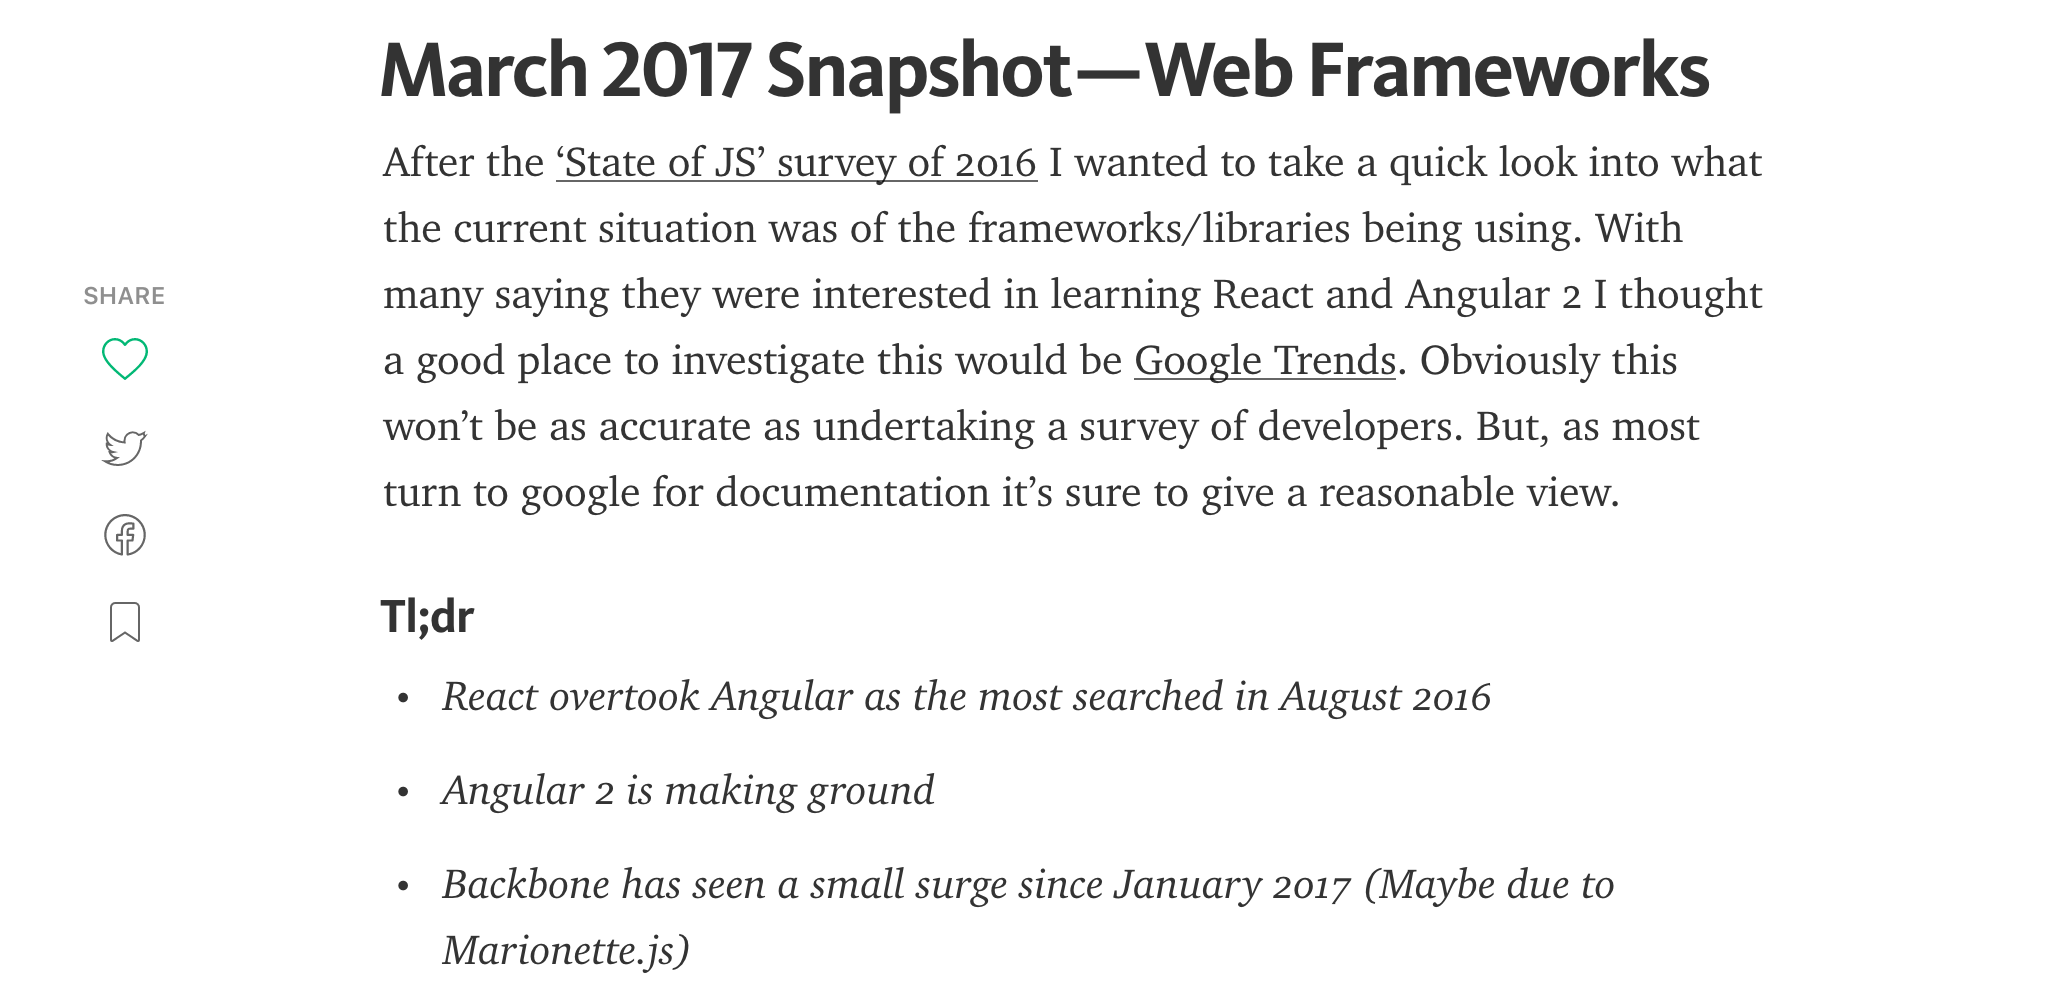
\includegraphics[width=0.65\textwidth]{figures/medium_example}
\captionsetup{justification=centering}
\caption{Diary Post on medium
\label{fig:medium_example}}
\end{figure}

Towards the end of the project these became less frequent and eventually
fizzled out due to the pressures around delivering the project.



\subsection{Planning}
At the start of my project I planned to use trello as a means of tracking what
needed to be done, what was in progress and what had been completed. My aim was
to use a kanban like approach and limit the work in progress to a single item.
In the hope of focussing me to work on a single thing at a time. After
initial setup though the board quickly became stale as I was mainly running
the project from a notepad which I was able to use in offline environments.

I felt that this turned out to be effective given my circumstances. Trello
just seemed to be hindering me. With a notepad I was able to
document thoughts, discussions and actions whilst at work. Where as with
trello I would have had to hold those until the end of the day before they
could be written down.

\subsection{Manifesto \& Methodology}
A manifesto was defined at the beginning of the project to help make
decisions and form an ethos for the project. Below I have documented where
each entry was used and its effect on the project.

\begin{center}
\textit{Making an impact over getting a good grade}
\end{center}
This was applied throughout the project. An example being the Colour Contrast
tool. I could have focussed on writing this report but instead created the
tool for assessing colour contrast. The tool is likely to add a limited amount
of value towards my grade but instead will offer other engineers a simple
effective means for assessing the colour contrast between a foreground and
background colour. The impact it made to date was demonstrated in
section \ref{sec:colour_contrast}

\begin{center}
\textit{Hypothesis’ and supporting evidence over guessing and assuming}
\end{center}
During the development of the A11Y guide this was followed extensively. For
example I hypothesised that React was the framework others were using and
then gained evidence to support the fact.

With the A11Y tool however a lot of assumptions were made and as a result I
believe the produce was not as good.

\begin{center}
\textit{``Start simple with many organic iterations" over ``Upfront design"}
\end{center}
Similar to above the A11Y Guide was the perfect example of this. THe
iterations were clearly defined and well planned. The content was produced
first, the web site on top of the content was then produced and each
iteration improved on the inital product.

I feel the A11Y tool was a bit more of a `big bang' approach. More upfront
design probably would have resulted in better defined iterations and maybe a
better product. It may have been the fact I had any preconceptions about what
I had from such a tool.

Fig.~\ref{fig:agile_bicycle} demonstrates this well. The A11Y Guide felt like
it followed the bottom image, the A11Y tool the top.

\begin{figure}[H]
\centering
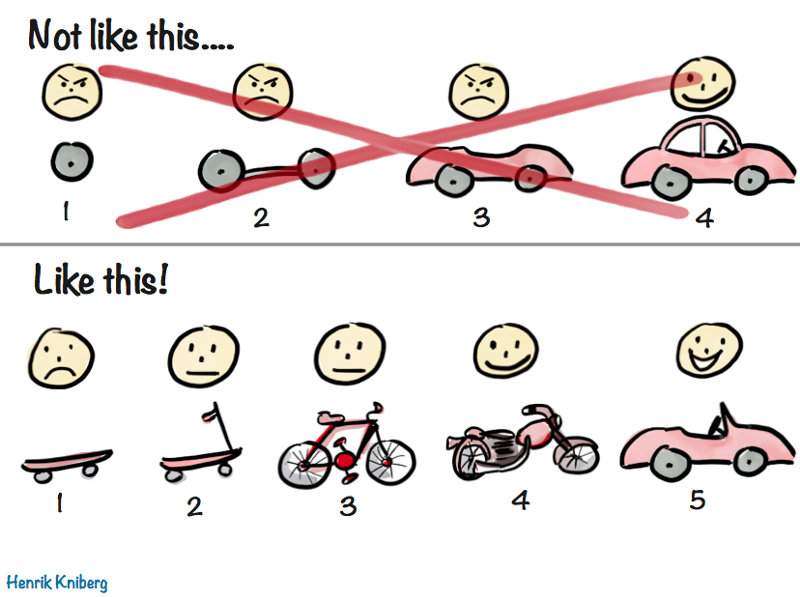
\includegraphics[width=0.6\textwidth]{figures/agile_bicycle}
\captionsetup{justification=centering}
\caption{The `Agile Bicycle' by \citep{bicycle}
\label{fig:agile_bicycle}}
\end{figure}

\subsubsection{Continuous delivery}
An aim of this project was to deliver products whilst they were still
undergoing active development. This has been successful. The A11Y guide, the
A11Y Tool and this very report were all produced using continuous delivery.
Although consumers may not have been using the deliverables it has been
extremely comforting to know that anything I change is tested and deployed
upon commit. Gone is the ``It worked on my machine'' and by using Github to
store the project I haven't had to worry about problems like my laptop
breaking losing internet. Fig.~\ref{fig:ghub} are the statistics for this
very report. A release in the report context is a `tag' at a point in the
github history at which a pdf has been produced.

\begin{figure}[H]
\centering
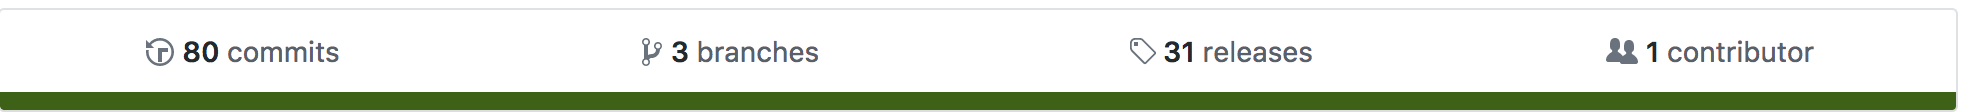
\includegraphics[width=0.8\textwidth]{figures/ghub}
\captionsetup{justification=centering}
\caption{Repository statistics for this very report
\label{fig:ghub}}
\end{figure}

\section{Personal reflections}
On a personal level I have en emense level of proudness surrounding what I
have delivered. I have become a subject matter expert in producing
accessibile web applications. I have diversified my knowledge in the area of
accessibility. I have experimented with some new ways of working. I have
networked with sought after members of the development community and I
have taken an idea and delivered it as a product. This project is a great
demonstration and culmination of some of the skills I have gained along my
journey as an apprentice.
